%---------------------
\pagestyle{plain}
\setcounter{page}{1}
\pagenumbering{arabic}
%---------------------

\chapter{مقدمه}

در این فصل به عنوان مقدمه، روش وارسی مدل و نظریه تعبیر مجرد، به‌طور مختصر، معرفی شده‌اند. در فصل‌های بعدی، با هدف بهبود روش وارسی مدل، صورت جدیدی از این روش ارائه شده و مورد بررسی قرار گرفته است، بنابراین لازم است که ابتدا، این دو موضوع معرفی شوند.

\section{روش وارسی مدل}

روش وارسی مدل یک روش صوری است که برای درستی‌یابی سیستم‌های مختلف استفاده می‌شود. در این روش معمولا ابتدا یک ماشین حالات متناهی از روی سیستم مورد بررسی ساخته می‌شود، سپس بررسی‌هایی که قرار است روی سیستم اصلی انجام شوند، روی این ماشین( مدل) انجام می‌شود. 

از این روش در بررسی صحت کارکرد برنامه‌های کامپیوتری استفاده می‌شود، اما این تنها مورد استفاده‌ی این روش نیست. و هر سیستمی که قابلیت بیان شدن به صورت صوری را داشته باشد، با این روش قابل بررسی است. مثلا می‌توان از این روش برای بررسی صحت عملکرد یک برنامه برای قطارهای شهری استفاده کرد. در یک برنامه‌ برای قطارهای شهری، نباید امکان حضور دو قطار روی یک ریل در یک زمان وجود داشته باشد( که معنی تصادف بین دو قطار را می‌دهد) و می‌توان از روش وارسی مدل برای اطمینان از عدم وجود چنین ویژگی نامطلوبی استفاده کرد. مثال های دیگر استفاده‌ی این روش در علوم کامپیوتر بررسی صحت عملکرد یک پردازنده یا الگوریتم تقسیمِ وظایف یک سیستم عامل است. این مثال‌ها هیچ کدام یک برنامه‌ی کامپیوتری نیستند( هر چند که ممکن است مجبور باشیم از یک برنامه‌ی کامپیوتری برای پیاده سازی آن‌ها کمک بگیریم که در آن صورت بررسی صحت عملکرد آن برنامه‌ی کامپیوتری داستانی دیگر خواهد داشت)، اما قابل بیان به صورت صوری به جای زبان طبیعی هستند.

روش وارسی مدل برای بیان خواص مورد بررسی از منطق‌های زمانی مختلف استفاده می‌کند. منطق زمانی یک نوع منطق موجهات است. منطق‌های موجهات از گسترش زبان منطق کلاسیک، با اضافه کردن ادات وجهی گوناگون، ساخته می‌شوند. این ادوات غالبا در زبان طبیعی نقش قید را دارند. منطق‌های زمانی دسته‌ای از منطق‌های موجهات هستند که به صوری‌گری ما مفهوم زمان را اضافه می‌کنند، یعنی قیدهایی مانند فعلا، بعدا، و قبلا( که مورد آخری کمتر رایج است). منطقی که در اینجا بیان می‌کنیم \lr{LTL} نام دارد که یکی از منطق‌های زمانی است که برای روش وارسی مدل استفاده می‌شود. البته در مورد قیدهای مذکور، اشاره به این نکته ضروری است که در بیانی که در اینجا از این منطق ارائه داده‌ایم، ادوات جدید به‌طور مستقیم بیانگر این قید‌ها نیستند، هرچند که به کمک ادوات جدید می‌توان ادواتی برای هر یک از این قیود ساخت.
این تعاریف از \cite{buchi} آورده شده‌اند.

ابتدا زبان این منطق را بیان می‌کنیم و سعی می‌کنیم، به طور غیر دقیق، در مورد معنای فرمول‌های این زبان به خواننده یک درک شهودی بدهیم، سپس به سراغ معناشناسی صوری این منطق می‌رویم.

\subsection{زبان \lr{LTL}}
\begin{defn}
	هر عضو مجموعه‌ی $\Phi$ یک فرمول در زبان \lr{LTL} است( و $\Pi$ مجموعه‌ی‌( شمارای نامتناهی) فرمول‌های اتمی است و $\pi \in \Pi$):
	$$
	\Pi \subset \Phi,
	$$
	$$
	\phi \in \Phi \Leftrightarrow
	\phi ::= \pi | \phi \lor \phi |
	\neg \phi |
	\bigcirc \phi |
	\phi \mathcal{U}\phi 
$$	
	
\end{defn}
در این منطق، ما زمان را با اعداد طبیعی نشان می‌دهیم. یعنی برای یک فرمول، زمان از عدد ۰ شروع شده و تا ابد ادامه خواهد داشت و حین گذر زمان ممکن است ارزش فرمول‌ها تغییر کند. مسلما پس از بررسی معناشناسی صوری بهتر می‌شود این مفهوم را به طور شهودی حس کرد، اما به هر حال به خواننده پیشنهاد می‌شود، پیش از رسیدن به آن بخش به ادامه‌ی این بخش که در تلاش است یک درک شهودی از معنای فرمول‌ها بدهد، توجه کند. 

در این زبان ادوات کلاسیک 
$\neg, \lor$
هستند با همان معنایی که در منطق گزاره‌ای کلاسیک داشتند.  
در ادوات جدید 
$\bigcirc \phi$
به معنای برقرار بودن این فرمول دقیقا در لحظه‌ی بعدی( دقیقا یک لحظه) است، مثلا در شکل زیر با در نظر گرفتن اینکه در زمان 0 هستیم، این فرمول در لحظه‌ی ۱ برقرار است.
	\begin{center}
	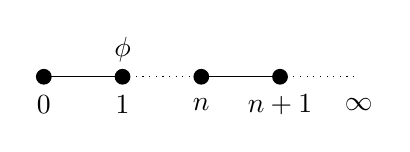
\begin{tikzpicture}
	\node at (1,0.35) (phi) {$\phi$};
	\node at (1,-0.35) (1) {$1$};
	\node at (0,-0.35) (0) {$0$};
	\node at (2,-0.35) (n) {$n$};
	\node at (3,-0.35) (1) {$n+1$};
	\node at (4,-0.35) (1) {$\infty$};
	\fill (0,0) circle (0.1cm);
	\fill (1,0) circle (0.1cm);
	\fill (2,0) circle (0.1cm);
	\fill (3,0) circle (0.1cm);
	\path (0,0) edge (1,0) 
	(1,0) edge[dotted] (2,0)
	(2,0) edge (3,0)
	(3,0) edge[dotted] (4,0);
	\end{tikzpicture}
\end{center}
$\phi \mathcal{U}\psi$
به این معنی است که فرمول سمت چپی حداقل تا قبل از اینکه فرمول سمت راستی برقرار شود، برقرار است.( مثلا اگر بگوییم "تا وقتی که باران نباریده زمین خشک است" در این صورت "زمین خشک است" به جای فرمول سمت چپ و "باران باریده است" فرمول سمت راست است).
\begin{center}
	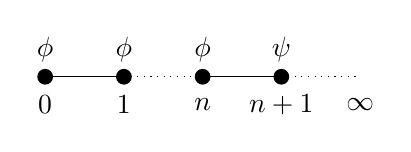
\begin{tikzpicture}
	\node at (1,0.35) (phi) {$\phi$};
	\node at (0,0.35) (phi) {$\phi$};
	\node at (2,0.35) (phi) {$\phi$};
	\node at (3,0.35) (phi) {$\psi$};
	\node at (1,-0.35) (1) {$1$};
	\node at (0,-0.35) (0) {$0$};
	\node at (2,-0.35) (n) {$n$};
	\node at (3,-0.35) (1) {$n+1$};
	\node at (4,-0.35) (1) {$\infty$};
	\fill (0,0) circle (0.1cm);
	\fill (1,0) circle (0.1cm);
	\fill (2,0) circle (0.1cm);
	\fill (3,0) circle (0.1cm);
	\path (0,0) edge (1,0) 
	(1,0) edge[dotted] (2,0)
	(2,0) edge (3,0)
	(3,0) edge[dotted] (4,0);
	\end{tikzpicture}
\end{center}

این زبان را می‌توان با ادوات بیشتری از آنچه آورده‌ایم بیان کرد و البته بیان‌های دیگری هم بسته به بحث متداول هستند، اما در اینجا یک شکل ساده از این زبان را آورده‌ایم که به غیر از ادوات منطق گزاره‌ای دو ادات دیگر را در زبان خود دارد. دلیل وجود ادوات متفاوت، می‌تواند راحت‌تر کردن بیان خواص باشد. همان طور که استفاده نکردن از یا و شرطی در منطق گزاره‌ای می‌تواند به سخت کردن بیان جملات در چارچوب این منطق منجر شود، حذف این ادوات وجهی هم بیان خواص را در این منطق مشکل می‌سازد. 

حال که به درکی شهودی از معنای فرمول‌های این زبان رسیده‌ایم، به بیان صوری این مفاهیم می‌پردازیم.

\subsection{معناشناسی \lr{LTL}}

مدل‌های این منطق را به صورت توابع
$M:\mathbb{N}_0 \rightarrow \mathit{P}(\Pi)$ 
تعریف می‌کنیم. به عبارت دیگر، هر مدل یک تابع است که هر عدد طبیعی را به یک مجموعه از فرمول‌های اتمی می‌برد. این در واقع به این معنی است که یک مدل مشخص می‌کند که در هر لحظه کدام یک از فرمول‌های اتمی درست هستند. مثلا، در مدلی به نام $M$ در واقع
$M(5)$
مجموعه‌ی اتم‌هایی است که در لحظه‌ی 5 طبق این مدل درست هستند و اگر اتمی در این مجموعه حاضر نباشد، در لحظه‌ی 5، ارزش غلط دارد.
درستی یک فرمول در یک مدل را با 
$M,i$
نشان می‌دهیم و 
$M,i \models \phi$
به این معنی است که فرمول $\phi$، در لحظه‌ی $i$در مدل $M$ ارزش درست دارد. این مفهوم را، به صورت بازگشتی، به شکل زیر تعریف می‌کنیم:


\begin{flushleft}
$	M,i \models \pi \:\:\: \mathit{iff} \:\:\: \pi \in M(i)$\\
$	M,i \models \neg \phi \:\:\: \mathit{iff} \:\:\: M,i\nvDash \phi$\\
$	M,i \models \phi \lor \psi \:\:\: \mathit{iff} \:\:\: M,i \models \phi \:\:\: \mathit{or} \:\:\: M,i \models \psi$\\
	 $M,i \models \bigcirc \phi  \:\:\:  \mathit{iff} \:\:\: M,i+1 \models \phi$\\
	 $M,i \models \phi \mathcal{U} \psi \:\:\: \mathit{iff} \:\:\: 
	 \exists k \geq i \in \mathbb{N}_0: \forall i\leq j< k: M,j \models \phi \:\:\: \mathit{and} \:\:\: M,k \models \psi$
\end{flushleft}


یک فرمول را ارضاپذیر می‌گوییم اگر و تنها اگر مدلی وجود داشته باشد که فرمول در آن صادق باشد.
اگر یک فرمول در هر مدلی صادق باشد، آن فرمول را \emph{معتبر} می‌گوییم.\\


\section{نظریه تعبیر مجرد}

به‌طور خلاصه، نظریه تعبیر مجرد یک چارچوب برای ساختن یک تقریب از معناشناسی یک زبان‌ برنامه نویسی است. 

معناشناسی یک زبان یک مدل ریاضیاتی مجرد است که چگونگی رفتار برنامه‌ها در این زبان را توصیف می‌کند. 
تقریب نیز یک معناشناسی دیگر است که قرار است بخشی( نه همه) از رفتارهای یک برنامه‌ی کامپیوتری در حال اجرا در یک زبان را توصیف کند. این که تقریب چیست، یک معناشناسی را در چه زمانی می‌توانیم تقریبی برای معناشناسی دیگری بدانیم و از یک تقریب چه چیزهایی را می‌توانیم بفهمیم و مواردی دیگر در مورد ارتباط بین دو مدل ریاضیاتی که درباره‌ی معنای برنامه‌ها در یک زبان برنامه‌نویسی واحد صحبت می‌کنند، همگی موضوع بحث در نظریه‌ي تعبیر مجرد است.
پس تا اینجا مشخص شد که نظریه‌ی تعبیر مجرد در مورد ارتباط بین معناشناسی‌های مختلف صحبت می‌کند. 

برای شروع بحث صوری در مورد این نظریه، از مفهوم دامنه و معناشناسی شروع می‌کنیم.
در واقع، این نوع از مشخص کردن معناشناسی یک زبان برنامه نویسی را معناشناسی دِلالَتی نامیده‌اند. در فصول آینده با یک معناشناسی از این نوع سر و کار خواهیم داشت.
\begin{defn}
	(معناشناسی و دامنه): اگر $\mathbb{P}$ مجموعه‌ی برنامه‌ها در یک زبان برنامه نویسی باشد، به تابع 
	$\mathcal{S}:\mathbb{P} \rightarrow D$
	یک معناشناسی و به مجموعه‌ی $D$ یک دامنه می‌گوییم.
\end{defn}
همان‌طور که از تعریف مشخص است، برای این که بتوانیم معنای برنامه‌های کامپیوتری موجود در یک زبان را تعریف کنیم، به یک مجموعه به اسم دامنه احتیاج داریم. تلاش برای پی بردن به این که در یک معناشناسی باید چه مجموعه‌ای را به عنوان دامنه در نظر گرفت، منجر به تولد یک مبحث به نام نظریه‌ی دامنه شده است.

در فصل‌های بعدی، با یک معناشناسی دلالتی سر و کار خواهیم داشت. 
پس از ارائه‌ی یک زبان برنامه نویسی، یک معناشناسی برای آن زبان معرفی می‌کنیم که معناشناسی رد پیشوندی نام دارد. در این معناشناسی، دامنه یک مجموعه است که شامل موجوداتی به نام رد پیشوندی است. هر رد پیشوندی یک دنباله است که در هر عضو آن اطلاعات موجود در حافظه و مرحله‌ی اجرای برنامه مشخص شده است. 

اما فعلا که در حال صحبت در مورد نظریه‌ی تعبیر مجرد هستیم، معناشناسی خاصی را معرفی نمی‌کنیم و بحث را کلی‌تر پیش می‌بریم. نظریه تعبیر مجرد برای معناشناسی‌ها یک چارچوب مشخص کرده و فقط در مورد معناشناسی‌هایی که در این چارچوب می‌گنجند می‌تواند صحبت کند. یکی از محدودیت‌های این چارچوب این است که دامنه باید یک ترتیب جزئی باشد.
\begin{defn}
	(ترتیب جزئی): یک مجموعه‌ی $D$ را به همراه یک رابطه‌ی $\leq$ روی آن مجموعه ترتیب جزئی می‌گوییم، اگر و تنها اگر خواص زیر را داشته باشند:
	$$\blacktriangleleft \forall a \in D: a\leq a$$
	$$\blacktriangleleft \forall a,b \in D: a \leq b \land b \leq a \rightarrow a=b$$
	$$\blacktriangleleft \forall a,b,c \in D: a \leq b \land b \leq c \rightarrow a \leq c$$
\end{defn}

حال به تعریف بخش بزرگتری از این چارچوب می‌پردازیم. در جبر مجرد مفهومی به اسم تناظر گالوا وجود دارد. این تناظر بین مجموعه‌ای از گروه‌ها و مجموعه‌ای از توسیع میدان‌هایی خاص وجود دارد که به بحث ما مربوط نمی‌شوند. این تناظر یک شکل نظریه ترتیبی هم دارد که در آن به جای مجموعه‌ای از گروه‌ها و میدان‌ها، دو مجموعه‌ی جزئا مرتب داریم. می‌توان گفت در واقع این یک مجرد سازی تناظری است که از جبر آمده. 

به شکل ضعیف‌تر نظریه ترتیبی این تناظر اتصال گالوا می‌گویند که در نظریه تعبیر مجرد به عنوان شرط تقریب تعریف شده است، به این معنی که دامنه‌ی یک معناشناسی باید با دامنه‌ی تقریبش یک اتصال گالوا داشته باشد.

\begin{defn}
	(اتصال گالوا): برای دو ترتیب جزئی
	$(A,\leq)$ 
	و
	$(C,\subseteq)$
	زوج 
	$\langle \alpha , \gamma \rangle$
	شامل دو تابع
	$\gamma:A \rightarrow C$
	و
	$\alpha:C \rightarrow A$،
	 یک اتصال گالوا است اگر و تنها اگر
	$$\forall c \in C :\forall a \in A: \alpha(c)\leq a \leftrightarrow c \subseteq \gamma(a)$$.
\end{defn}







